\documentclass[11pt,a4paper]{article}
\usepackage[utf8]{inputenc}
\usepackage[vietnamese]{babel}
\usepackage{amsmath,amssymb}
\usepackage[version=4]{mhchem}
\usepackage{geometry}
\geometry{top=0.9cm,bottom=0.9cm,left=1.35cm,right=1.35cm,headheight=24pt,headsep=5pt,footskip=11pt}
\usepackage{graphicx}
\usepackage{xcolor}
\usepackage{tabularx}
\usepackage{array}
\usepackage{tikz}
\usepackage{multicol}
\usepackage{fancyhdr}
\usepackage{enumitem}

\definecolor{hfRed}{HTML}{D32F2F}
\definecolor{hfGreen}{HTML}{8BC390}
\definecolor{mainGreen}{HTML}{2E7D32}

\usepackage{ex_test}

\pagestyle{fancy}
\fancyhf{}
\renewcommand{\headrulewidth}{0.75pt}
\renewcommand{\headrule}{\hbox to\headwidth{\color{hfGreen}\leaders\hrule height \headrulewidth\hfill}}
\renewcommand{\footrulewidth}{0.75pt}
\renewcommand{\footrule}{\hbox to\headwidth{\color{hfGreen}\leaders\hrule height \footrulewidth\hfill}}

\fancyhead[L]{\small\itshape\color{hfRed}Tài liệu lưu hành nội bộ}
\fancyhead[R]{\small\color{hfRed}Thầy \textbf{TRẦN VĂN THẠNH} - 0777.470.803}

\fancyfoot[L]{\footnotesize\itshape\color{hfRed}CS1: 6/15 Nguyễn Hoàng, P. Kim Long, TP Huế \quad|\quad CS2: 24 Đặng Thái Thân, TP Huế}
\fancyfoot[R]{\small\textbf{\color{hfRed}Trang \thepage}}

\setlength{\parindent}{0pt}
\setlength{\parskip}{1.2pt}

\def\loigiai#1{
\par\begingroup\color{blue!80!black}\small
\noindent\textbf{\textit{Lời giải chi tiết:}}\par
#1\par\endgroup}

\begin{document}
\Opensolutionfile{ans}[ans-de16-gv]

\noindent
\begin{minipage}[t]{0.48\textwidth}
	\textbf{SỞ GIÁO DỤC VÀ ĐÀO TẠO THỪA THIÊN HUẾ}\\
	\textbf{TRƯỜNG THPT HAI BÀ TRƯNG}\\
	\textbf{ĐỀ CHÍNH THỨC}\\
	\textit{(Đề thi có 04 trang)}
\end{minipage}\hfill
\begin{minipage}[t]{0.48\textwidth}
	\raggedleft
	\textbf{\color{mainGreen}ĐỀ KIỂM TRA ĐỊNH KỲ CHƯƠNG 6 (ĐẠI CƯƠNG KIM LOẠI)}\\
	\textbf{MÔN: HOÁ HỌC -- LỚP 12}\\
	\textit{Thời gian làm bài: 50 phút (không kể thời gian phát đề)}\\
	\textbf{Mã đề thi: 116}
\end{minipage}


\vspace{0.1cm}
\begin{center}
	\textbf{\color{hfRed}\Large (BẢN GIÁO VIÊN -- CÓ LỜI GIẢI CHI TIẾT)}
\end{center}

\vspace{1pt}
\noindent\textit{Họ, tên thí sinh: \dots\dots\dots\dots\dots\dots\dots\dots\dots\dots\dots\dots\dots\dots\dots\dots\dots\dots\dots\dots\dots\dots Lớp: \dots\dots\dots\dots SBD: \dots\dots\dots\dots}\\
\noindent\textit{(Cho biết nguyên tử khối: H = 1; C = 12; N = 14; O = 16; Na = 23; Mg = 24; Al = 27; S = 32; Cl = 35,5; K = 39; Ca = 40; Cr = 52; Fe = 56; Cu = 64; Zn = 65; Sn = 119; Ag = 108; Pt = 195; Au = 197; Pb = 207; hằng số Faraday F = 96500 C/mol).}

\vspace{2pt}
\noindent
\textbf{PHẦN I (4,5 điểm -- 18 câu): Câu trắc nghiệm nhiều phương án lựa chọn.}\\
\textit{Thí sinh trả lời từ câu 1 đến câu 18. Mỗi câu hỏi thí sinh chỉ chọn một phương án.}

\setcounter{ex}{0}

\begin{ex}
Phát biểu nào sau đây về tinh thể kim loại là đúng?
\choice
{Chứa các cation kim loại và các electron hoá trị. Chúng cùng chuyển động tự do trong tinh thể.}
{Chứa các cation kim loại và nguyên tử kim loại có tương tác tĩnh điện với nhau.}
{\True Chứa các cation kim loại sắp xếp theo trật tự nhất định và các electron hoá trị chuyển động tự do.}
{Bao gồm các cation kim loại và electron hoá trị tự do. Giữa chúng hình thành liên kết ion giúp tinh thể kim loại có cấu trúc bền vững.}
\loigiai{
Mạng tinh thể kim loại gồm các cation kim loại nằm ở các nút mạng tinh thể sắp xếp theo một trật tự xác định và các electron hoá trị tự do chuyển động trong toàn bộ mạng tinh thể.\\
\textbf{Chọn C.}}
\end{ex}

\begin{ex}
Lực liên kết kim loại gây ra bởi
\choice
{\True tương tác tĩnh điện giữa cation kim loại và electron hoá trị tự do trong tinh thể.}
{sự góp chung các electron hoá trị giữa các nguyên tử kim loại trong tinh thể.}
{tương tác van der Waals giữa các nguyên tử kim loại trong tinh thể.}
{sự hình thành liên kết cho -- nhận giữa các nguyên tử kim loại trong tinh thể.}
\loigiai{
Liên kết kim loại là liên kết được hình thành do lực hút tĩnh điện giữa các cation kim loại ở nút mạng tinh thể và các electron hoá trị tự do chuyển động trong tinh thể.\\
\textbf{Chọn A.}}
\end{ex}

\begin{ex}
Tính chất vật lí chung của kim loại được quyết định bởi
\choice
{bán kính nguyên tử kim loại.}
{\True các electron hoá trị tự do trong tinh thể kim loại.}
{kiểu tinh thể kim loại.}
{độ âm điện của nguyên tử kim loại.}
\loigiai{
Các tính chất vật lí chung của kim loại (tính dẻo, tính dẫn điện, tính dẫn nhiệt và ánh kim) đều do các electron tự do trong mạng tinh thể kim loại gây ra.\\
\textbf{Chọn B.}}
\end{ex}

\begin{ex}
Hai kim loại thường được dùng làm dây dẫn điện là
\choice
{\True đồng (copper) và nhôm (aluminium).}
{đồng (copper) và tungsten.}
{nhôm (aluminium) và sắt (iron).}
{kẽm (zinc) và nhôm (aluminium).}
\loigiai{
Đồng và nhôm là hai kim loại có độ dẫn điện tốt, giá thành hợp lí và độ bền cao nên được sử dụng phổ biến nhất để chế tạo dây dẫn điện.\\
\textbf{Chọn A.}}
\end{ex}

\begin{ex}
Trong môi trường có $\text{pH} = 7$, các kim loại tan trong nước thường có giá trị thế điện cực chuẩn
\choice
{lớn hơn $-0{,}413\text{ V}$.}
{\True nhỏ hơn $-0{,}413\text{ V}$.}
{lớn hơn $-0{,}826\text{ V}$.}
{nhỏ hơn $-0{,}826\text{ V}$.}
\loigiai{
Ở $\text{pH} = 7$ (môi trường trung tính), thế điện cực của quá trình khử nước ($\ce{2H2O + 2e <=> H2 + 2OH-}$) là $E = -0{,}413\text{ V}$. Để kim loại khử được nước giải phóng $\ce{H2}$ ở điều kiện này, thế điện cực chuẩn của cặp oxi hoá -- khử kim loại phải nhỏ hơn $-0{,}413\text{ V}$.\\
\textbf{Chọn B.}}
\end{ex}

\begin{ex}
Trong quá trình tái chế kim loại, ở công đoạn phân loại phế liệu, có thể dùng nam châm lớn để tách riêng phế liệu
\choice
{nhôm (aluminium).}
{\True thép.}
{đồng (copper).}
{kẽm (zinc).}
\loigiai{
Thép có thành phần chính là sắt (Fe) có tính nhiễm từ mạnh (bị nam châm hút), do đó có thể dùng nam châm điện lớn để tách riêng phế liệu thép khỏi các kim loại khác.\\
\textbf{Chọn B.}}
\end{ex}

\begin{ex}
Xỉ xuất hiện trong quá trình tách kim loại, luyện kim và tinh luyện để tái chế kim loại. Xỉ là hỗn hợp nhiều chất, hỗn hợp này thường
\choice
{\True có khối lượng riêng nhỏ hơn so với khối lượng riêng của kim loại cần tách hoặc cần tái chế.}
{dễ chảy lỏng.}
{dễ bay hơi.}
{có nhiều độc tính nên cần phải được chôn lấp sau khi được tháo ra khỏi lò.}
\loigiai{
Xỉ lò (như \ce{CaSiO3},\dots) có khối lượng riêng nhỏ hơn kim loại lỏng nên nổi lên bề mặt, giúp dễ dàng gạt bỏ và bảo vệ kim loại lỏng không bị oxi hoá bởi không khí.\\
\textbf{Chọn A.}}
\end{ex}

\begin{ex}
Hợp kim là
\choice
{một kim loại tinh khiết.}
{hỗn hợp các kim loại có thành phần tùy ý.}
{\True hỗn hợp của kim loại nền với kim loại khác hoặc phi kim, có thành phần xác định.}
{hỗn hợp hai phi kim.}
\loigiai{
Hợp kim là vật liệu kim loại chứa một kim loại cơ bản (kim loại nền) và một số kim loại khác hoặc phi kim, có thành phần xác định nhằm cải thiện cơ tính.\\
\textbf{Chọn C.}}
\end{ex}



\begin{ex}
Kim loại cơ bản trong dural và thép 304 lần lượt là
\choice
{nhôm và magnesium.}
{\True nhôm và sắt.}
{magnesium và sắt.}
{kẽm và sắt.}
\loigiai{
Dural (duralumin) có kim loại cơ bản là nhôm ($\ce{Al} > 90\%$); Thép 304 (inox 304) có kim loại cơ bản là sắt (Fe).\\
\textbf{Chọn B.}}
\end{ex}

\begin{ex}
Thành phần quan trọng của inox là
\choice
{\True sắt (iron), chromium, carbon.}
{nhôm (aluminium), magnesium.}
{đồng (copper), kẽm (zinc).}
{sắt (iron), magnesium, carbon.}
\loigiai{
Inox (thép không gỉ) có thành phần chính là sắt kết hợp với chromium (tối thiểu $10{,}5\%$ tạo màng thụ động chống gỉ), carbon và nickel.\\
\textbf{Chọn A.}}
\end{ex}

\begin{ex}
Sự ăn mòn kim loại
\choice
{là sự phá hủy kim loại hoặc hợp kim do các chất điện li trong môi trường.}
{chính là sự ăn mòn điện hoá.}
{diễn ra trong dung dịch chất điện li.}
{\True là sự phá huỷ kim loại hoặc hợp kim do tác dụng của các chất trong môi trường, trong đó kim loại bị oxi hoá.}
\loigiai{
Định nghĩa: Sự ăn mòn kim loại là sự phá huỷ kim loại hoặc hợp kim do tác dụng hoá học hoặc điện hoá của các chất trong môi trường, trong đó kim loại bị oxi hoá.\\
\textbf{Chọn D.}}
\end{ex}

\begin{ex}
Phát biểu nào dưới đây là \textbf{không đúng} về chống ăn mòn kim loại?
\choice
{Phủ lên bề mặt của kim loại một lớp sơn, dầu, mỡ, chất dẻo hoặc tráng, mạ bằng một kim loại khác là những cách chống ăn mòn kim loại theo phương pháp phủ bề mặt.}
{Nối kim loại cần bảo vệ với một kim loại hoạt động hoá học mạnh hơn là cách chống ăn mòn kim loại theo phương pháp điện hoá.}
{\True Quấn một dây kẽm quanh đinh sắt là cách để chống ăn mòn kẽm trong môi trường có chất điện li.}
{Để tránh ăn mòn đồ trang sức bằng Ag thì người ta thường phải đánh sạch hoặc rửa sạch trong xà phòng.}
\loigiai{
Quấn dây kẽm quanh đinh sắt là phương pháp điện hoá để bảo vệ đinh sắt (kẽm bị ăn mòn thay cho sắt), không phải để chống ăn mòn kẽm. Nhận định C sai.\\
\textbf{Chọn C.}}
\end{ex}

\begin{ex}
Ở phản ứng tách kim loại từ zinc oxide bằng phương pháp nhiệt luyện tạo ra
\choice
{\True kẽm (zinc) ở thể hơi.}
{kẽm (zinc) và hơi nước.}
{kẽm (zinc) ở thể rắn.}
{hợp kim của zinc và carbon.}
\loigiai{
Phản ứng: $\ce{ZnO + C -> Zn + CO}$ (ở nhiệt độ $> 1000^\circ\text{C}$). Do kẽm có nhiệt độ sôi $907^\circ\text{C}$ nên ở nhiệt độ này kẽm thoát ra ở thể hơi, sau đó được ngưng tụ thu hồi.\\
\textbf{Chọn A.}}
\end{ex}

\begin{ex}
Phát biểu nào sau đây là đúng khi nói về phương pháp tách kim loại ra khỏi hợp chất của chúng?
\choice
{Đồng có thể được tách từ copper(II) oxide bằng cách nung nóng.}
{\True Kim loại Zn được tách ra khỏi ZnO bằng phương pháp nhiệt luyện.}
{Kim loại Mg được tách ra khỏi dung dịch \ce{MgCl2} bằng phương pháp điện phân.}
{Kim loại Al được tách ra khỏi \ce{Al2O3} bởi CO bằng phương pháp nhiệt luyện.}
\loigiai{
ZnO bị khử bởi C hoặc CO ở nhiệt độ cao thu được kim loại Zn (phương pháp nhiệt luyện). Các phát biểu còn lại đều sai.\\
\textbf{Chọn B.}}
\end{ex}

\begin{ex}
Phát biểu nào sau đây là \textbf{không đúng} về điều kiện xảy ra ăn mòn điện hoá?
\choice
{Hai điện cực phải tiếp xúc trực tiếp hoặc thông qua dây dẫn.}
{Hai điện cực cùng tiếp xúc với dung dịch chất điện li.}
{\True Hai điện cực phải là hai kim loại khác loại.}
{Thiếu một trong các điều kiện về điện cực, tiếp xúc, chất điện li sẽ không xảy ra ăn mòn.}
\loigiai{
Hai điện cực có thể là một kim loại và một phi kim dẫn điện (ví dụ: Fe và C trong gang, thép), không bắt buộc phải là hai kim loại khác loại. Nhận định C sai.\\
\textbf{Chọn C.}}
\end{ex}

\begin{ex}
Trong lò luyện gang có phản ứng: $\ce{Fe2O3 + 3CO -> 2Fe + 3CO2}$. Để tăng hiệu suất phản ứng, có thể sử dụng các biện pháp nào sau đây?
\choice
{Tăng diện tích bề mặt \ce{Fe2O3}.}
{\True Tăng lượng khí CO, giảm lượng khí \ce{CO2}.}
{Giảm áp suất chung của hệ phản ứng.}
{Tăng áp suất chung của hệ phản ứng.}
\loigiai{
Tăng nồng độ chất phản ứng (CO) và liên tục loại bỏ sản phẩm (\ce{CO2}) làm cân bằng chuyển dịch mạnh mẽ theo chiều thuận, làm tăng hiệu suất phản ứng.\\
\textbf{Chọn B.}}
\end{ex}

\begin{ex}
Dural là một loại hợp kim quan trọng của nhôm, có đặc điểm là nhẹ, cứng, bền cơ học phù hợp với các ứng dụng nào sau đây?\\
(1) Chế tạo cánh máy bay. \quad (2) Áo giáp, khiên bảo vệ. \quad (3) Làm ống dẫn dầu, mỏ neo.
\choice
{(1), (2).}
{\True (1).}
{(1), (2), (3).}
{(1), (3).}
\loigiai{
Duralumin có độ bền cao và rất nhẹ, ứng dụng chủ yếu trong chế tạo vỏ, cánh máy bay và phương tiện giao thông. Ống dẫn dầu hay mỏ neo cần vật liệu chịu ăn mòn biển sâu hoặc nặng như thép đúc.\\
\textbf{Chọn B.}}
\end{ex}

\begin{ex}
Các tấm tôn (thép mạ kẽm) lợp nhà thường bị gỉ sét nhanh hơn tại các vị trí cố định bằng đinh thép. Nguyên nhân của hiện tượng này là do
\choice
{việc đóng đinh tạo điều kiện cho nước mưa tiếp xúc với các kim loại trong tấm tôn.}
{đinh thép đóng vai trò như anode làm cho việc ăn mòn diễn ra nhanh hơn.}
{\True do trong đinh thép có carbon, đóng vai trò như cathode thúc đẩy quá trình ăn mòn.}
{do chất lượng thép của đinh và trong tấm tôn là không đồng nhất.}
\loigiai{
Khi đóng đinh thép, carbon trong đinh thép đóng vai trò là cathode (cực dương), tiếp xúc với màng nước mưa làm tăng tốc độ ăn mòn điện hoá của lớp kẽm và lõi thép tôn.\\
\textbf{Chọn C.}}
\end{ex}



\noindent
\textbf{PHẦN II (4,0 điểm -- 4 câu): Câu trắc nghiệm đúng sai.}\\
\textit{Thí sinh trả lời từ câu 1 đến câu 4. Trong mỗi ý a), b), c), d) ở mỗi câu, thí sinh chọn đúng hoặc sai.}

\setcounter{ex}{0}

\begin{ex}
Kim loại magnesium có khối lượng riêng là $1{,}74\text{ g/cm}^3$. Kim loại này phản ứng chậm với nước ở nhiệt độ thường tạo ra anion \ce{OH-} và khí \ce{H2}, phản ứng nhanh với sulfuric acid loãng và làm nhạt màu dung dịch copper(II) sulfate. Mỗi phát biểu sau đây là đúng hay sai?
\choiceTF
{Những hợp kim mà magnesium đóng vai trò kim loại cơ bản là những hợp kim nặng.}
{Giá trị thế điện cực chuẩn của \ce{Mg^2+/Mg} lớn hơn 0 V.}
{\True Trong môi trường trung tính, có: $\ce{2H2O + 2e <=> 2OH- + H2}$ với $E = -0{,}413\text{ V}$.}
{\True Giá trị thế điện cực chuẩn của \ce{Cu^2+/Cu} lớn hơn giá trị thế điện cực chuẩn của \ce{Mg^2+/Mg}.}
\loigiai{
a) \textbf{Sai}. Magnesium có khối lượng riêng nhỏ ($1{,}74\text{ g/cm}^3 < 5\text{ g/cm}^3$) nên là kim loại nhẹ, hợp kim của nó là hợp kim nhẹ.\\
b) \textbf{Sai}. $E^\circ_{\ce{Mg^2+/Mg}} = -2{,}37\text{ V} < 0\text{ V}$.\\
c) \textbf{Đúng}. Trong môi trường trung tính ($\text{pH} = 7$), thế khử của nước là $-0{,}413\text{ V}$.\\
d) \textbf{Đúng}. $E^\circ_{\ce{Cu^2+/Cu}} = +0{,}34\text{ V} > E^\circ_{\ce{Mg^2+/Mg}} = -2{,}37\text{ V}$.}
\end{ex}

\begin{ex}
Cho lá kim loại kẽm (zinc) vào ống nghiệm chứa lượng dư dung dịch copper(II) sulfate màu xanh, thấy:\\
-- Màu xanh của dung dịch nhạt dần.\\
-- Có hiện tượng sủi bọt khí quanh lá kim loại.\\
Mỗi phát biểu sau đây là đúng hay sai?
\choiceTF
{Tính oxi hoá của \ce{Zn^2+} mạnh hơn tính oxi hoá của \ce{Cu^2+}.}
{\True Trong ống nghiệm có diễn ra quá trình ăn mòn điện hoá.}
{Muối \ce{ZnSO4} không tan trong nước.}
{Trong ống nghiệm có diễn ra quá trình các ion \ce{H+} nhận electron.}
\loigiai{
a) \textbf{Sai}. Tính oxi hoá của \ce{Cu^2+} mạnh hơn \ce{Zn^2+}.\\
b) \textbf{Đúng}. Kim loại Cu sinh ra bám vào Zn tạo cặp điện cực Zn -- Cu cùng tiếp xúc với dung dịch chất điện li $\Rightarrow$ xảy ra ăn mòn điện hoá học.\\
c) \textbf{Sai}. \ce{ZnSO4} là muối tan tốt trong nước.\\
d) \textbf{Sai}. Quá trình nhận electron chủ đạo là của ion \ce{Cu^2+} ($\ce{Cu^2+ + 2e -> Cu}$).}
\end{ex}

\begin{ex}
\begin{minipage}[t]{0.65\textwidth}
Hình bên minh hoạ quá trình tinh chế đồng bằng phương pháp điện phân. Mỗi phát biểu sau đây là đúng hay sai?
\begin{enumerate}[label=\alph*),leftmargin=1.5em,itemsep=0pt,topsep=1pt]
	\item \textbf{\color{red}[ĐÚNG] }Thanh A là đồng nguyên chất, thanh B là đồng chứa tạp chất.
	\item \textbf{\color{red}[ĐÚNG] }C là dung dịch \ce{CuSO4}.
	\item \textbf{\color{red}[SAI] }D là đồng tinh khiết.
	\item \textbf{\color{red}[SAI] }Thanh đồng B nối vào cực âm của nguồn điện.
\end{enumerate}
\end{minipage}\hfill
\begin{minipage}[t]{0.33\textwidth}
	\centering
	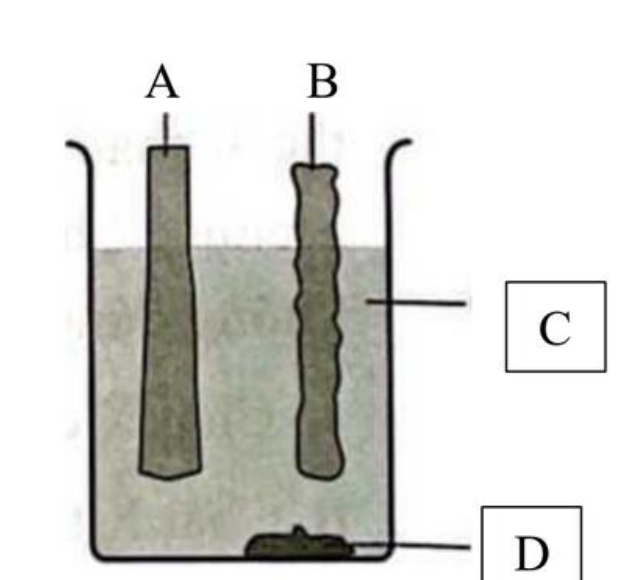
\includegraphics[width=\linewidth]{images_crop_de16/p2_cau3_tinh_che_dong.png}
\end{minipage}
\loigiai{
a) \textbf{Đúng}. Thanh A là cathode (đồng tinh khiết, đồng bám vào dày lên), thanh B là anode (đồng thô chứa tạp chất, tan dần).\\
b) \textbf{Đúng}. Dung dịch C là chất điện li \ce{CuSO4}.\\
c) \textbf{Sai}. D là bùn anode lắng dưới đáy chứa các tạp chất không tan như Ag, Au, Pt.\\
d) \textbf{Sai}. Thanh B là anode chứa tạp chất nên phải nối vào cực dương của nguồn điện.}
\end{ex}

\begin{ex}
Trong vỏ Trái đất, sắt và nhôm là hai nguyên tố kim loại có hàm lượng cao hơn so với các nguyên tố kim loại khác. Mỗi phát biểu sau đây là đúng hay sai?
\choiceTF
{Sắt hoặc nhôm đều được sử dụng với vai trò là kim loại cơ bản trong sản xuất các hợp kim nặng.}
{Từ quặng bauxite sẽ tách được sắt bằng phương pháp nhiệt luyện, từ quặng hematite sẽ tách được nhôm bằng phương pháp điện phân.}
{Khi tráng một lớp kẽm lên đinh thép sẽ hạn chế được sự ăn mòn sắt trong thép theo phương pháp điện hoá.}
{\True Nhiệt độ cần để tái chế thép cao hơn nhiệt độ cần để tái chế nhôm.}
\loigiai{
a) \textbf{Sai}. Nhôm là kim loại nhẹ dùng làm hợp kim nhẹ.\\
b) \textbf{Sai}. Quặng bauxite dùng để điều chế nhôm, quặng hematite dùng để luyện gang, thép (sắt).\\
c) \textbf{Sai}. Tráng kẽm là phương pháp bảo vệ bề mặt.\\
d) \textbf{Đúng}. Nhiệt độ nóng chảy của Fe ($1538^\circ\text{C}$) cao hơn nhiều so với Al ($660^\circ\text{C}$).}
\end{ex}



\noindent
\textbf{PHẦN III (1,5 điểm -- 6 câu): Câu trắc nghiệm yêu cầu trả lời ngắn.}\\
\textit{Thí sinh trả lời từ câu 1 đến câu 6.}

\setcounter{ex}{0}

\begin{ex}
Cho quá trình: $\ce{4Al(s) + 3O2(g) -> 2Al2O3(s)}$, $\Delta_{\text{r}} H^\circ_{298} = -3351{,}4\text{ kJ}$. Lượng nhiệt toả ra khi 1 gam nhôm (aluminium) bị oxi hoá hoàn toàn ở điều kiện chuẩn là bao nhiêu kJ? (Làm tròn kết quả đến hàng phần mười).
\par\noindent\textbf{Đáp số:} \textbf{\color{red}31,1}
\loigiai{
Theo phương trình nhiệt hoá học, 4 mol Al (tương ứng $4 \times 27 = 108\text{ g}$) toả ra $3351{,}4\text{ kJ}$.\\
Nhiệt lượng toả ra khi oxi hoá hoàn toàn 1 gam nhôm là:
$$Q = \frac{3351{,}4}{108} \approx 31{,}03 \approx 31{,}1\text{ kJ.}$$
\textbf{Đáp số: 31,1.}}
\end{ex}

\begin{ex}
Cho các kim loại: Ag, Al, Au, Cu, Cr, Fe, Mg, Pt, Zn. Có bao nhiêu kim loại phản ứng được với dung dịch sulfuric acid đặc, nguội?
\par\noindent\textbf{Đáp số:} \textbf{\color{red}4}
\loigiai{
-- Au, Pt là kim loại trơ không phản ứng với \ce{H2SO4} đặc, nguội.\\
-- Al, Fe, Cr bị thụ động hoá trong \ce{H2SO4} đặc, nguội.\\
-- Các kim loại phản ứng được gồm: Ag, Cu, Mg, Zn. Tổng cộng có 4 kim loại.\\
\textbf{Đáp số: 4.}}
\end{ex}

\begin{ex}
Cho các cặp oxi hoá -- khử: \ce{Ag+/Ag}, \ce{Al^3+/Al}, \ce{Au^3+/Au}, \ce{Cu^2+/Cu}, \ce{Fe^2+/Fe}, \ce{K+/K}, \ce{Mg^2+/Mg}, \ce{Na+/Na}, \ce{Pt^2+/Pt}, \ce{Zn^2+/Zn} và \ce{Pb^2+/Pb}. Có bao nhiêu cặp oxi hoá -- khử có giá trị thế điện cực chuẩn lớn hơn 0 V?
\par\noindent\textbf{Đáp số:} \textbf{\color{red}4}
\loigiai{
Các cặp oxi hoá -- khử có $E^\circ > 0\text{ V}$ đứng sau \ce{H+/H2} trong dãy điện hoá gồm:\\
\ce{Cu^2+/Cu} ($+0{,}34\text{ V}$), \ce{Ag+/Ag} ($+0{,}80\text{ V}$), \ce{Pt^2+/Pt} ($+1{,}20\text{ V}$), \ce{Au^3+/Au} ($+1{,}52\text{ V}$).\\
Tổng cộng có 4 cặp.\\
\textbf{Đáp số: 4.}}
\end{ex}

\begin{ex}
Có bao nhiêu trường hợp xảy ra ăn mòn điện hoá trong các quá trình sau?\\
(a) Vỏ tàu bằng thép có gắn các khối kẽm, neo đậu tại một cảng biển.\\
(b) Vật dụng bằng bạc bị sẫm màu khi tiếp xúc với không khí có lẫn \ce{H2S}.\\
(c) Tấm tôn trầy xước trên mái nhà tiếp xúc với nước mưa.\\
(d) Hợp kim Na -- K nóng đỏ, bốc cháy khi tiếp xúc với khí chlorine.\\
(e) Một cổ vật làm bằng đồng thau (hợp kim Cu -- Zn) chìm trong nước biển.\\
(g) Dây chảy cầu chì làm bằng hợp kim Pb -- Sn đứt khi cường độ dòng điện tăng đột ngột.
\par\noindent\textbf{Đáp số:} \textbf{\color{red}3}
\loigiai{
Các trường hợp ăn mòn điện hoá gồm:\\
-- (a) Cặp Zn -- Fe trong chất điện li nước biển.\\
-- (c) Cặp Zn -- Fe bị trầy xước tiếp xúc với màng nước mưa.\\
-- (e) Cặp Cu -- Zn trong hợp kim đồng thau tiếp xúc với nước biển.\\
Các trường hợp (b), (d) là ăn mòn hoá học; (g) là hiện tượng vật lý.\\
Tổng cộng có 3 trường hợp.\\
\textbf{Đáp số: 3.}}
\end{ex}

\begin{ex}
Trong quá trình sản xuất nhôm (aluminium) bằng phương pháp điện phân nóng chảy \ce{Al2O3}, điện cực dương bằng than chì bị ăn mòn liên tục do phản ứng tạo thành hỗn hợp khí \ce{O2}, CO, \ce{CO2} có tỉ lệ mol bằng nhau. Giả sử các phản ứng xảy ra hoàn toàn, mỗi kg nhôm sinh ra tương ứng với bao nhiêu kg than chì bị đốt cháy ở cực dương? (Làm tròn đến hàng phần trăm).
\par\noindent\textbf{Đáp số:} \textbf{\color{red}0,27}
\loigiai{
Gọi số mol các khí ở anode: $n_{\ce{O2}} = x$, $n_{\ce{CO}} = x$, $n_{\ce{CO2}} = x\text{ (kmol)}$.\\
Tổng mol nguyên tử $\ce{O} = 2x + x + 2x = 5x\text{ kmol} \Rightarrow n_{\ce{Al}} = \frac{10x}{3}\text{ kmol}$.\\
Khối lượng Al: $m_{\ce{Al}} = \frac{10x}{3} \times 27 = 90x = 1\text{ kg} \Rightarrow x = \frac{1}{90}\text{ kmol}$.\\
Khối lượng carbon bị đốt cháy:
$$m_{\ce{C}} = 12 \times (n_{\ce{CO}} + n_{\ce{CO2}}) = 12 \times 2x = 24 \times \frac{1}{90} \approx 0{,}267 \approx 0{,}27\text{ kg.}$$
\textbf{Đáp số: 0,27.}}
\end{ex}

\begin{ex}
Một dòng điện 1,04 A đi qua dung dịch sulfuric acid loãng trong 6,00 phút trong một thiết bị điện phân nước. Tổng số mol \ce{H2} và \ce{O2} thu được là $n \times 10^{-3}\text{ mol}$. Giá trị của $n$ là bao nhiêu? (Làm tròn kết quả đến hàng phần trăm).
\par\noindent\textbf{Đáp số:} \textbf{\color{red}2,91}
\loigiai{
-- Thời gian: $t = 6{,}00 \times 60 = 360\text{ giây}$.\\
-- Số mol electron trao đổi:
$$n_e = \frac{I \times t}{F} = \frac{1{,}04 \times 360}{96500} \approx 0{,}0038798\text{ mol.}$$
-- Quá trình ở các điện cực:\\
Cathode: $\ce{2H+ + 2e -> H2} \Rightarrow n_{\ce{H2}} = \frac{n_e}{2}$.\\
Anode: $\ce{2H2O -> O2 + 4H+ + 4e} \Rightarrow n_{\ce{O2}} = \frac{n_e}{4}$.\\
-- Tổng số mol khí:
$$n_{\text{khí}} = \frac{3}{4} n_e = \frac{3}{4} \times 0{,}0038798 \approx 0{,}00291\text{ mol} = 2{,}91 \times 10^{-3}\text{ mol.}$$
Giá trị của $n$ là 2,91.\\
\textbf{Đáp số: 2,91.}}
\end{ex}


\Closesolutionfile{ans}

\vspace{0.5cm}
\begin{center}
	\textbf{\Large\color{mainGreen}BẢNG TỔNG HỢP ĐÁP ÁN ĐỀ SỐ 16}
\end{center}

\vspace{0.2cm}
\noindent\textbf{\color{mainGreen}PHẦN I: TRẮC NGHIỆM NHIỀU PHƯƠNG ÁN LỰA CHỌN}
\begin{center}
\renewcommand{\arraystretch}{1.2}
\begin{tabular}{|c|c|c|c|c|c|c|c|c|c|c|c|c|c|c|c|c|c|}
\hline
\textbf{1} & \textbf{2} & \textbf{3} & \textbf{4} & \textbf{5} & \textbf{6} & \textbf{7} & \textbf{8} & \textbf{9} & \textbf{10} & \textbf{11} & \textbf{12} & \textbf{13} & \textbf{14} & \textbf{15} & \textbf{16} & \textbf{17} & \textbf{18} \\ \hline
\textbf{\color{red}C} & \textbf{\color{red}A} & \textbf{\color{red}B} & \textbf{\color{red}A} & \textbf{\color{red}B} & \textbf{\color{red}B} & \textbf{\color{red}A} & \textbf{\color{red}C} & \textbf{\color{red}B} & \textbf{\color{red}A} & \textbf{\color{red}D} & \textbf{\color{red}C} & \textbf{\color{red}A} & \textbf{\color{red}B} & \textbf{\color{red}C} & \textbf{\color{red}B} & \textbf{\color{red}B} & \textbf{\color{red}C} \\ \hline
\end{tabular}
\end{center}

\vspace{0.3cm}
\noindent\textbf{\color{mainGreen}PHẦN II: TRẮC NGHIỆM ĐÚNG SAI}
\begin{center}
\renewcommand{\arraystretch}{1.2}
\begin{tabular}{|c|c|c|c|c|}
\hline
\textbf{Câu} & \textbf{Lệnh hỏi a} & \textbf{Lệnh hỏi b} & \textbf{Lệnh hỏi c} & \textbf{Lệnh hỏi d} \\ \hline
\textbf{1} & \textbf{S} & \textbf{S} & \textbf{\color{red}Đ} & \textbf{\color{red}Đ} \\ \hline
\textbf{2} & \textbf{S} & \textbf{\color{red}Đ} & \textbf{S} & \textbf{S} \\ \hline
\textbf{3} & \textbf{\color{red}Đ} & \textbf{\color{red}Đ} & \textbf{S} & \textbf{S} \\ \hline
\textbf{4} & \textbf{S} & \textbf{S} & \textbf{S} & \textbf{\color{red}Đ} \\ \hline
\end{tabular}
\end{center}

\vspace{0.3cm}
\noindent\textbf{\color{mainGreen}PHẦN III: TRẢ LỜI NGẮN}
\begin{center}
\renewcommand{\arraystretch}{1.2}
\begin{tabular}{|c|c|c|c|c|c|}
\hline
\textbf{Câu 1} & \textbf{Câu 2} & \textbf{Câu 3} & \textbf{Câu 4} & \textbf{Câu 5} & \textbf{Câu 6} \\ \hline
\textbf{\color{red}31,1} & \textbf{\color{red}4} & \textbf{\color{red}4} & \textbf{\color{red}3} & \textbf{\color{red}0,27} & \textbf{\color{red}2,91} \\ \hline
\end{tabular}
\end{center}

\end{document}
